53. \begin{figure}[ht!]
\center{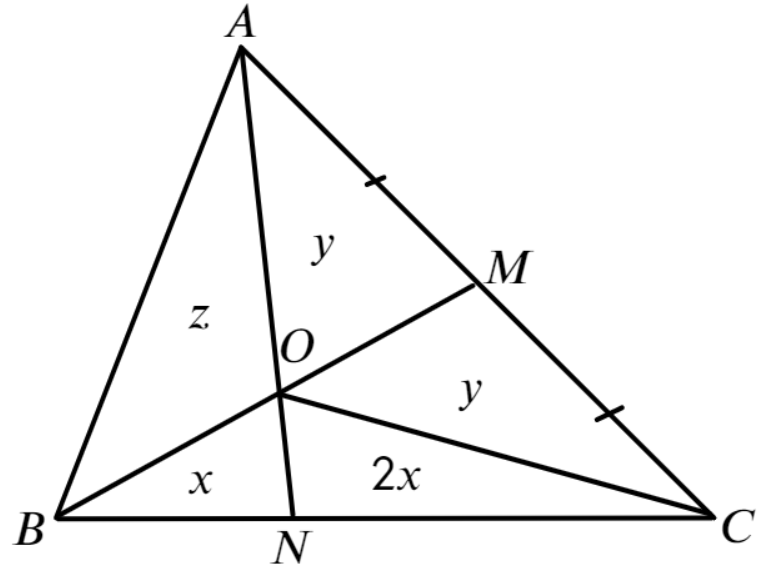
\includegraphics[scale=0.35]{g9-53.png}}
\end{figure}\\
Воспользовавшись тем, что площади треугольников, имеющих общую высоту, относятся как основания, на которые она опущена, введём обозначения: $S_{\Delta OBN}=x,\ S_{\Delta OCN}=2x,\ S_{\Delta AOM}=S_{\Delta COM}=y,\ S_{\Delta AOB}=z.$ Тогда так как $S_{\Delta ABM}=S_{\Delta CBM},$ имеем равенство $z+y=3x+y,$ откуда $z=3x.$ Так как $S_{\Delta ACN}=2S_{\Delta ABN},$ получим соотношения $(3x+x)\cdot2=2y+2x,\ y=3x.$ Так как $S_{\Delta ABO}=S_{\Delta AOM}=3x,$ получаем $BO:OM=1:1,$ а так как $\cfrac{S_{\Delta ABO}}{S_{\Delta BON}}=3,$ получаем $AO:ON=3:1.$\\
